\documentclass{beamer}
\usepackage{import}
\subimport{template/latex/settings/}{settings-pres}
\graphicspath{{images/}}
\usetheme{Warsaw}

\begin{document}

\title{Обзор библиотек для работы с нейронными сетями}
\author{Александр Мелихов}
\institute{Волгоградский государственный технический университет}
\date{Волгоград, 2015}

% Создание заглавной страницы.
\frame{\titlepage}

\begin{frame}{Решаемая задача}
    Решить, выдавать ли клиенту кредит или нет. Обучающая выборка взята из
    репозитория реальных данных, содержит 20 входных параметров, в числе которых:
    \begin{itemize}
        \item сумма кредита
        \item срок кредита
        \item кредитная история
        \item пол
        \item возраст и т. д.
    \end{itemize}
\end{frame}

\begin{frame}{AlgLib}
    Порядок работы с нейронной сетью:
    \begin{itemize}
        \item Выбрать конфигурацию нейронной сети (количество скрытых слоев (0,
            1 или 2), сжимающую функцию активации выходного слоя)
        \item Обучить нейронную сеть одним из следующих алгоритмов:
            \begin{itemize}
                \item L-BFGS
                    \begin{itemize}
                        \item Лучше всего подходит для решения задач высокой
                            размерности
                        \item Критерием останова служат малая величина шага или
                            превышение заданного числа итераций алгоритма
                    \end{itemize}
                \item модифицированный метод Левенберга-Марквардта
                    \begin{itemize}
                        \item Лучше на задачах мелкой и средней размерности
                        \item Не нуждается в критерии останова
                    \end{itemize}
                \item метод раннего останова (для ансамбля нн)
            \end{itemize}
    \end{itemize}
\end{frame}

\begin{frame}{AlgLib}
    Порядок работы с нейронной сетью:
    \begin{itemize}
        \item Подобрать параметры сети, подходящие для решаемой задачи
            (результаты проверяются с помощью кросс-валидации или тествого
            множества):
            \begin{itemize}
                \item Количество итераций алгоритма
                \item Количество рестартов со случайной позиции (затем
                    выбирается лучший результат)
                \item Количество скрытых слоев
                \item Значение шага
                \item Коэффициент регуляризации (от 0.001 до 100)
            \end{itemize}
        \item Использовать
    \end{itemize}
\end{frame}

\begin{frame}{AlgLib}
    Дополнительные возможности:
    \begin{itemize}
        \item Кросс-валидация (оценка способности нн к обобщению)
        \item Предобработка данных (стандартизация обучающего множества для
            улучшения скорости сходимости и качества получаемых значений)
    \end{itemize}
\end{frame}

\begin{frame}{AlgLib}
    Формат обучающего множества:
    \begin{itemize}
        \item Для задачи классификации:
            \begin{itemize}
                \item Первые N столбцов независимые параметры, остальные —
                    зависимые
            \end{itemize}
        \item Для задачи регрессии:
            \begin{itemize}
                \item Первые N столбцов независимые параметры, затем идет номер
                    первого класса, затем второго\ldots
            \end{itemize}
    \end{itemize}
\end{frame}

\begin{frame}{AlgLib}
    Кодирование номинальных переменных:
    \begin{itemize}
        \item номинальные переменные, принимающие два значения, кодируются
            одним числом - как «0» или как «1»
        \item номинальные переменные, принимающие три и более значения,
            кодируются с использованием схемы «1-of-N» (например, «красный»,
            «желтый» и «зеленый» можно закодировать, как «1 0 0», «0 1 0»,
            «0 0 1»).
        \item номинальная переменная, независимо от числа принимаемых значений,
            может быть закодирована целым числом (0, 1, 2, ..., N). Однако
            желательно, чтобы значения могли быть осмысленно упорядочены
            («холод», «комнатная температура», «жара»)
    \end{itemize}
\end{frame}

\begin{frame}{PyBrain}
    \begin{center}
        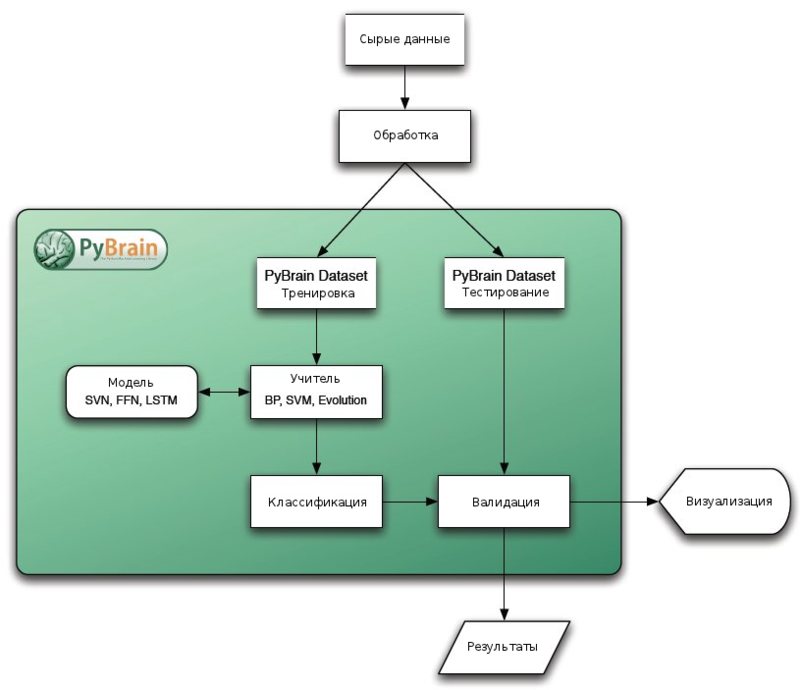
\includegraphics[width=100mm,height=70mm]{pybrain}
    \end{center}
\end{frame}

\begin{frame}{PyBrain}
    Особенности:
    \begin{itemize}
        \item Большое количество алгоритмов для обучения с учителем, без
            учителя, с подкреплением и для оптимизации методом черного ящика
        \item Большое количество функций активации
        \item Построение различных топологий сетей:
            \begin{itemize}
                \item Сети прямого распространения
                \item Рекурентные нейронные сети
                \item Сети Кохонена
                \item Создание топологий собственной структуры
            \end{itemize}
        \item Можно настроить практически любой параметр нн
    \end{itemize}
\end{frame}

\begin{frame}{Заключение}
    Плюсы AlgLib:
    \begin{itemize}
        \item Доступна на нескольких языках, кроссплатформенность, собирается
            почти любым компилятором
        \item В коммерческой версии реализовано распараллеливание алгоритмов и
            SSE оптимизации
    \end{itemize}
    Плюсы PyBrain:
    \begin{itemize}
        \item Настраиваимость практически любомого параметра нн
    \end{itemize}
    Минусы PyBrain:
    \begin{itemize}
        \item Плохо развивается, большое количество нерешенных issue
    \end{itemize}
\end{frame}

\end{document}
